%%%%%%%%%%%%%%%%%%%%%%%%%%% SEM-IMAC_template.tex %%%%%%%%%%%%%%%%%%%%%%%%%%%%%%%%%
%%% This is a template for the IMAC (International Modal Analysis Conference) style
%%% 
%%% This was developed by Austin R.J Downey for SEM-IMAC, last updated September 2024.
%%% Checked with MikTex on a Windows Machine for IMAC 2024. 
%%% Checked with Tex Live on a Linux Machine for IMAC 2025. 
%%% The repository associated with this template can be found at https://github.com/austindowney/SEM-IMAC-LaTeX-Template
%%% This work is licensed under a Creative Commons Attribution-ShareAlike 4.0 International License [cc-by-sa 4.0].
%%% 
%%%%%%%%%%%%%%%%%%%%%%%%%%%%%%%%%%%%%%%%%%%%%%%%%%%%%%%%%%%%%%%%%%%%%%%%%%%%%%%%%%%

\documentclass[10pt,letterpaper]{article}
\usepackage[left=0.75in, right=0.75in, top=0.75in, bottom=1.00in]{geometry}
\usepackage{mathptmx}				% needed for time font
\usepackage[hidelinks]{hyperref}	% added for inline hyperlinks
\usepackage[english]{babel}			% added for filler text
\usepackage{blindtext}				% added for filler text
\usepackage{graphicx}				% added for figures
\setlength{\parindent}{0em} 		% remove the indent for all paragraphs
\setlength{\parskip}{1em}			% septs the spacing between paragraphs
\usepackage{booktabs}				% added for tables
\usepackage{caption}				% added for figure captions
\captionsetup{justification=raggedright,singlelinecheck=false}	% left align figure captions
\usepackage{float}					% added to allow [H] for figures
\usepackage{amsmath}				% added for fonts
\usepackage{amsfonts}				% added for fonts
\usepackage{cite}					% added to allow for ranges in a list of citations
\usepackage{nopageno} 				% added to remove page numbers 


\makeatletter
\newcommand{\removeperiod}{\@ifnextchar.{\@gobble}\relax}		% added to help with removing the period after the year.
\makeatother

% Adjust the font and style of the title and author section.
\usepackage{etoolbox}
\makeatletter
\patchcmd{\@maketitle}{\Large}{\Large}{\typeout{OK 1}}{\typeout{Failed 1}}
\patchcmd{\@maketitle}{\large \lineskip}{\large \lineskip}{\typeout{OK 2}}{\typeout{Failed 2}}
\makeatother

% Set the section headers, no subsections defined.
\usepackage[explicit]{titlesec}
\renewcommand{\thesection}{}
\titleformat{\section}
  {\normalfont}{\thesection}{0pt}{\MakeUppercase{\textbf{#1}}}
\titlespacing*{\section}
  {0pt}{5ex}{-1em}

% Build the keyword command.
\newcommand{\keywords}[1]{\vspace{2ex} \noindent \textbf{Keywords:} #1}



%%%%%%%%%%%%%%%%%%%%%%%%%%%%%%%%%%%%%%%%%%%%%%%%%%%%%%%%%
%%% Start of the document
%%% 


\begin{document}
	\date{} % Keeps the date from being printed.
	
	% A short descriptive title of your work.
	\title{\LaTeX\  Template for the International Modal Analysis Conference (IMAC)}
	
	% List the authors of the work. 
	\author{\vspace{.25in}\\
	Austin Downey$^1$, Babe the Blue Ox$^2$, and Paul Bunyan$^3$\\ \\ % place a double line break after authors
	 $^1$Department of Mechanical Engineering \\
		University of South Carolina, Columbia, SC 29208 \\ \\ % place a double line break between institutions
	 $^2$Department of Farm Animal Health \\
	 $^3$Department of Forestry and Environmental Science \\
		North American Forestry University, New Town, WI 55401 \\
	}
	\maketitle
	
	% Include a short abstract at the beginning of the submission.
	\section{abstract}
		This is a \LaTeX\ template for SEM-IMAC. To use, simply replace the text in this template file with your publication. \href{https://github.com/austindowney/SEM-IMAC-LaTeX-Template}{The GitHub repository page can be found at https://github.com/austindowney/SEM-IMAC-LaTeX-Template}. Questions related to the \LaTeX\ document should be directed there. No promises are made in terms of timely help from the author.
	
	\keywords{Keyword One, Keyword Two, Keyword Three, Keyword Four, Keyword five - Note:All manuscripts must include 5 keywords}
	
	\section{Introduction}
	
		Every good paper needs to cite some prior work from IMAC \cite{Downey2021OpenVibrations,Singh2021RealTimeForecasting,Downey2020Millisecondmodelupdating,Downey2016HighCapacityVariable}, but should also reference figures and equations in the text. For example, Figure~\ref{fig:suspension} shows an image of a car suspension that is in the public domain. The displacement of the time can be modeled as a 1-DOF system as shown in equation~\ref{eq:1-DOF}.
		\begin{equation}
		m\ddot{x} + c\dot{x} + kx = F
		\label{eq:1-DOF}
		\end{equation}
		SEM IMAC does not want indentation for each paragraph. So the \LaTeX template takes care of that. Just make sure to have a space between new paragraphs but do not add spacing between equations you want to be included in a paragraph. 
		
		\begin{figure}
			\centering
			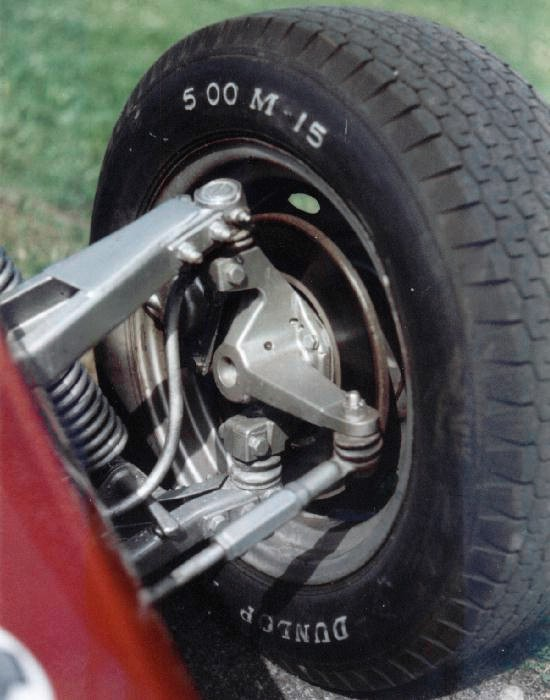
\includegraphics[width=2in]{papernum_dow_Fig1.jpg}
			\caption{A public domain picture of car suspension that is designed for vibration control.}
			\label{fig:suspension}
		\end{figure}
		
		This is a new paragraph so there is a space between it and the prior text. Good papers may also have tables, \href{https://www.tablesgenerator.com/}{the website tablesgenerator.com} is a great way to build tables.  
		\begin{table}[]
			\centering
			\caption{Results for a fictional test.}
			\label{table:test}
			\begin{tabular}{@{}lccccccc@{}}
				\toprule
				 & test 1 & test 2 & test 3 & test 4 & test 5 & test 6 & test 7 \\ \midrule
				metric 1 & 0.9 & 0.6 & 0.8 & 0.4 & 0.3 & 0.6 & 0.3 \\
				metric 2 & 1 & 12 & 5 & 32 & 8 & 32 & 2 \\ \bottomrule
			\end{tabular}
		\end{table}
		
		
		\blindtext
	
	
	\section{background}
		\blindtext
	
	\section{ANALYSIS}
		\blindtext
	
	\section{CONCLUSION}
		\blindtext
	
	\section{ACKNOWLEDGEMENTS}
		\blindtext
	
	\section{References}
		\vspace{-1.5ex}
		\bibliographystyle{imac_2021.bst}
		\renewcommand{\refname}{}
		\bibliography{imac}

\end{document}
